\chapter{Model-View-Controller for Science}\label{chapter:mvcs}

\section{Introduction}
Developing a computer program is much more than having few scripts that you can run when you need. A program should take care of a lot of concerns, such as the limits of the devices, should be flexible enough that enables you to change what measurements you are doing without spending months. More importantly, a program should be extensible in the long run, not just by yourself but also by future colleagues and, potentially, by anyone who find your program online.

Therefore, when we develop software, we want to keep in mind the following programmer's \emph{mantras}:

\begin{itemize}
\item What you develop should be readable by current and future colleagues
\item It should be easy to add solutions developed by others
\item The program should allow exchanging devices that achieve the same goal (i.e. oscilloscopes of different brands, etc.)
\item The code developed in one context has to be available in other contexts (i.e. in other experiments)
\end{itemize}

The first line does not pose a challend to be understood. When we talk about solutions developed by others, we mean that often times someone already wrote a driver for a device, or they wrote a measurement script. Therefore, it should be easy to get other's code and use them in our own projects. Exchanging devices is something that is not valued until it happens. In most labs there is always a legacy device that sooner or later will break down and will need to be replaced. Or you move to a different lab and need to continue with your experiments with different hardware. We will see strategies in the program to allow easy exchange of devices. Finally, when we talk about context, we mean that sometimes experiments are very different, but the logic behind is very similar. We are measuring the I-V curve of a diode, but it is, by no means, any different from doing a 1-D scan on a confocal microscope, or tuning the wavelength of a laser.

The mantras are not rules. They are just points on which you have to reflect in order to realize whether you are departing from the path you wanted to follow when you started. In the following sections we are going to explore a design pattern for software that has many benefits when developing scientific software for controlling experiments, it is called \textbf{The Model-View-Controller for Science}

\section{The MVCs design pattern}\label{section:MVC}
\begin{center}
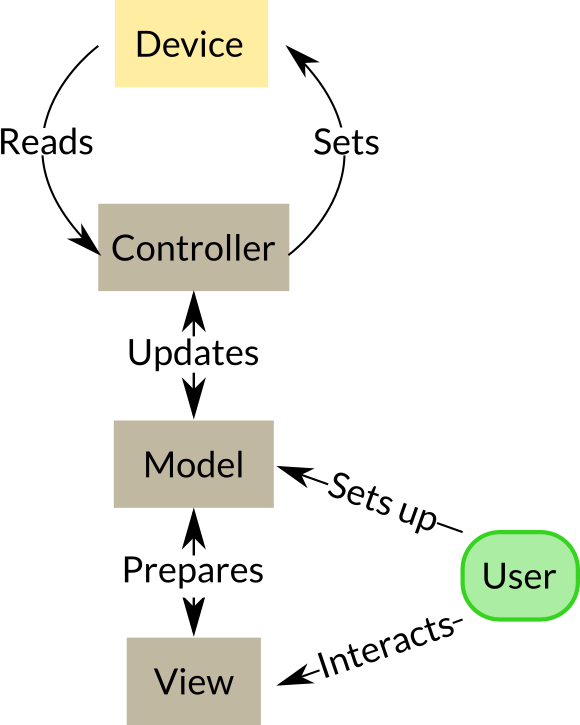
\includegraphics{images/Chapter_04/MVCs.png}
\end{center}

A design pattern is nothing more than a set of rules that determine where different parts of the code are going to be placed and how are they going to interact with each other. One of such patterns is called the Model-View-Controller, or MVC for short. When you work with devices in the lab, there is an extra layer that most computer programs lack, which is the interaction with the real world through specific devices. That is why we decided to nickname the pattern MVCs, with the s for \emph{science}. Let's see what each component of the MVC is about.

A \emph{Controller} for our purposes can also be called \emph{a driver}, which is responsible for communicating with devices. It can be a Python class we developed ourself such as the one we did in the previous chapter, but it can also be a Python package developed by someone else. The latter scenario is the case when manufacturers provide the drivers themselves, such as PyPylons from Basler, or the NI-DAQmx bindings for Python. The driver has to reflect the capabilities of the device, nothing less and nothing more. For example, if a device is able to acquire just a data point at a time, the driver shouldn't include a function for acquiring an array of data using a loop. We briefly discussed this in the previous chapter. Whatever belongs to the logic that a user imposes belongs to Model component.

The \emph{Model} is where all the logic is defined. In the models, we are going to define how we are going to use a device for our own experiment. A clear example would be the introduction of units. The device from the previous chapter takes only integer values as inputs. If we would like to transform that input to voltages, we could do it in the model for the device. Moreover, one of the analog  inputs is measuring a voltage, but it can be transformed to a current. This is very specific to our experiment and thus the option shouldn't be hardcoded in the driver. The place to include this information is the model. The main advantage of splitting \emph{Controllers} and \emph{Models} is that it becomes simple to upgrade or replace a device. You will need to update the \emph{Model} in order to reflect the new options of the device, but the logic of the experiment is left intact.

There is a second type of model, which is the \emph{Experiment Model}, in which we link different devices in order to perform a measurement. Or we use a single device, but we add the features that an experiment needs, for example saving data, plotting, analysing, etc. With very simple examples, the boundary between the device model and the experiment model can be blurry, but when you are dealing with several devices or more complex flows, it becomes much clearer. At the end of the book we will give as a reference some projects we have worked on, that can be a good source of inspiration.

The \emph{View} is the place where you can locate everything related to how you show data to the user, and how the user can change the parameters of the experiment. In practice, it is the collection of files that build up a Graphical User Interface ({GUI}). Within the {GUI} you will set, for example, the start, stop, and step of the experiment. This information will be passed to the model to acquire the data. You can plot the results back to the user and save them to disk, etc. It is important to note that, in this case, the user interacts through the view with the model and never directly with the controller of a device. It is also important to keep in mind that all the logic of what you are developing should be implemented in the model. For example, if you save the data to files, the procedure to create new filenames should be specified in the Model and not in the View.

For our project, the controller is what we discussed on Chapter \ref{chapter:first-driver}, the model for the device will be discussed on Chapter \ref{chapter:device-model}, the model for the experiment on Chapter \ref{chapter:experiment-model}, and the view will be discussed in Chapters \ref{ch:gui} and \ref{ch:user-input}. As you can see, there are still a lot of things to cover in the book. It is important to be patient, because we are going to grow a solution slowly, based on need, and solving the mistakes that may appear as we go, and not just following blindly a path.

\warning{If you are new to developing code for the lab, it may hard to understand why and how to split \emph{Controller} and \emph{Model}. When you have only one device that you use for only one goal and that is as simple is the device we are using in this book, the differences between model and controller are very thin. However, when you wish to include code developed by others or when you want to share your code, it is crucial that you split the capabilities of your device from the logic of your experiment. If you don't do so, all your code is going to work only when doing just one, very specific, experiment.}

The meaning of \emph{Model}, \emph{View} and \emph{Controller} changes depending on each developer or community. People developing a web application are not dealing with devices in the real world as developers in the lab do. Therefore, the {MVC} pattern definition can change from one field to another. The details are not that important, once we establish a structure, if we follow it, everyone else will be able to understand quickly what the code is doing and where. Once we understand what each different component is, we will very quickly understand where we need to change the code in order to solve a bug or add new functionality.

\section{Structure of The Program}\label{section:structure-of-theprogram}
In the program we are developing in this book, we will follow the MVC design pattern quite literally. This means that we have to create three folders called \emph{Model}, \emph{View} and \emph{Controller}. In the previous chapter, we have already developed the driver for the device. Go ahead and move the file \textbf{pftl\_daq.py} into the Controller folder.

\exercise{Create a file \textbf{analog\_daq.py} in the Models. Inside the file, define a class called \mintinline{python}{AnalogDaq} what methods do you think that belong to the device Model?}

In our definition of Model, it is important to make a further distinction. On the one hand, we have models for the devices we use. In those models, we will define things such as units, how to initialize the device, etc. However, experiments often require to perform complex tasks in which several devices are synchronized. When we perform an experiment we will need to save the data or load the configuration from a file.

\exercise{Create a file in the Models folder, called \textbf{experiment.py}. Define a class called \mintinline{python}{Experiment} and add some methods that you think are going to be useful. You can, for example, add a method for switching on or off the {LED}. You can also add a method for doing a scan of an analog output signal. The methods can be empty, don't worry about making it work, but just about the layout. You have to start thinking about the parameters that you need and the order in which every method can be called. For example, to save the data, you will need to specify a folder.}

The View folder is going to require a bit more of work than the other two. However, you can already start thinking about how the user is going
to interact with your program. Most likely, you have already thought that sometimes the {LED} will be plugged into the output channel number 1,
sometimes to channel number 0. You don't want to change the code every time you change where you plugged the LED. The same happens, for example, with the channel you want to monitor, the time delay between steps, etc. All this behavior will be included in the view in the last chapters of the book.

Now that you have started to split the code into different folders and files, it is important to discuss how can you make programs that use the code available in different files. That is called \emph{importing} and is the focus of the next section.

\section{Importing modules in Python}\label{section:importing-python}
In the previous chapter, we have already seen some lines that look like this:

\begin{minted}{python}
import numpy as np
from time import sleep
\end{minted}

The first one is importing the numpy package, but changing its name to \mintinline{python}{np}. Changing the name makes it easier to work with because you need to type only two letters, \mintinline{python}{np} instead of \mintinline{python}{numpy}. The second line is importing one specific function from a package called \mintinline{python}{time}. It is important to realize that the import process was different in both cases. \emph{Numpy} is a complex package, with a lot of modules that can be used. The same is true for \emph{time}. However, in the lines above we have imported only the module \emph{sleep} from package \emph{time}. If we want to use it, we can do:

\begin{minted}{python}
sleep(1)
\end{minted}

While for using \emph{Numpy}, we will need to specify which module we want:

\begin{minted}{python}
np.random.random(1)
\end{minted}

If we know we only want to use \mintinline{python}{random} from \emph{Numpy}, we can also import and use it like this:

\begin{minted}{python}
from numpy.random import random

random(1)
\end{minted}

We may wonder why we would import all of numpy is you are just using one of its functions. The name \emph{random} is not defined solely by numpy. Python also provides its own random module. We can import it like this:

\begin{minted}{python}
import random
\end{minted}

If we needed both \emph{random} functions in the same program, we would have a clash. How would we be sure we are using Numpy's and not Python's function? We may, for example, define our own random function and we would like to be able to choose which one to use and, more importantly, we want to avoid generating an unexpected behavior because of redefining functions without realizing it.

When working with our own code, we can import different modules in the same way. Open a terminal and navigate to the root folder of the project, i.e. the folder that contains the Model, View, and Controller folders. Start the Python interpreter, and then type:

\begin{minted}{pycon}
>>> from Controller.pftl_daq import Device
\end{minted}

Now we have the controller available to use. We can do the following:

\begin{minted}{pycon}
>>> dev = Device('/dev/ttyACM0')
>>> dev.initialize()
\end{minted}

However, there is something strange happening if we actually run the code above. As soon as we import \texttt{Device}, it will actually start communicating with the device and will output the identification number, and will switch on and off the LED. This is, of course, something we don't want, and a very common pitfall for Python developers. Of course, we don't want to trigger a measurement just because we imported the module to our program.

To avoid running code when importing, we must change the file \textbf{pftl\_daq.py}. We can add one line of code at the end of the file, and some indentation, to make it look like this:

\begin{minted}{python}
if __name__ == "__main__":
    dev = Device('/dev/ttyACM0') #<---- Remember to change the port
    dev.initialize()
    serial_number = dev.idn()
    print(f'The device serial number is: {serial_number}')
    for i in range(10):
        dev.set_analog_output(0, 4000)
        volts = dev.get_analog_input(0)
        print(f'Measured {volts}')
        sleep(.5)
        dev.set_analog_output(0, 0)
        volts = dev.get_analog_input(0)
        print(f'Measured {volts}')
        sleep(.5)
\end{minted}

To see the changes, we first must close python running the \texttt{exit()} command, and then opening it again. Python does not import twice the same modules, and therefore, it won't realize that the file with our controller changed. After we restart Python, we can try again importing the controller. Now things are going to look fine, and we will be able to use the \texttt{Device} as we intended. The best idea is to leave the space at the bottom of the files only with examples on how to use what we have just developed. If we ever find the Device around, and we don't remember what we were supposed to do with it, we can always go to the bottom of the file and see how it works.

Every time we encounter a behavior which is not easy to understand, the best idea is to transform it into simpler components and explore them one by one. In this case, the importing process may be a bit confusing. To understand it a bit more about, especially how the \mintinline{python}{if __name__} works we can create a new file called \textbf{dummy\_controller.py} in the \emph{Controller} folder, with the following lines of code:

\begin{minted}{python}
print('This is the dummy Controller')

def dummy_example():
    print('This is a function in the dummy Controller')

if __name__ == '__main__':
    print('This is printed only from __main__')
    dummy_example()

\end{minted}

From the terminal, we can just type \texttt{python Controller.dummy\_controller.py}. The output should be:

\begin{minted}{bash}
'This is the dummy Controller'
'This is printed only from __main__'
'This is a function in the dummy Controller'
\end{minted}

What we see is that the entire code got executed.

\exercise{What do you expect to happen if you do \mintinline{python}{import dummy_controller}?}

Things are going to be different when we import the file. In the Python interpreter we can do the following:

\begin{minted}{pycon}
>>> import dummy_controller
"This is the dummy Controller"
>>> dummy_controller.dummy_example()
"This is a function in the dummy Controller"
>>> from dummy_controller import dummy_example
>>> dummy_example()
"This is a function in the dummy Controller"
\end{minted}

First we notice that the code at the end never gets executed. This means that the \texttt{if} statement is not \texttt{True}. This is very useful when we want to have code that works standalone (when we execute it directly, for example) but we don't want to execute those lines if we import it. In the case of the real controller, we wanted to leave some examples at the end to show how it can be used, but when we are importing a class, we don't really want it to start communicating with the device.

We can also see that the line \texttt{"This is the dummy Controller"} appears only once. Python knows that we have already imported the module \textbf{dummy\_controller} and it doesn't execute again the lines that were already executed. Therefore, we have to be aware that it is not a matter of using the \texttt{from} in the importing procedure. We can close Python, start it again and revert the order in which we import and the print will still be there the first time but not the second. This means that Python is very smart when importing modules, and won't fetch the elements it already has available, even if we are importing in a slightly different way.

\note{We should establish some naming conventions in order to avoid confusion later on. In Python, any file that defines variables, functions, classes, etc. is called a \mintinline{python}{Module}. The folder that contains modules is called a \mintinline{python}{Package}.}

Working with the imports in Python is sometimes easier than understanding them, especially when trying to pay attention to all the different definitions. The \href{https://docs.python.org/3.6/tutorial/modules.html}{Python Documentation} has a great chapter covering a lot of the ideas discussed. Many of the properties and behaviors can be learned by trial and error, though it can be very time consuming and it may lead to unexpected errors.

There is one final remark that is worth mentioning about packages. Right now, we have three folders in our project: Model, View, and Controller. But what would happen if we add a new folder called, for example, \emph{serial}. Next time we try to do \texttt{import serial}, how would Python know if it is supposed to import the PySerial library or our own package? It can also happen the other way around, perhaps we don't know there is something already called \emph{Controller} in Python, and we don't care about it, we want to import our own modules.

In order for Python to understand that a folder is meant to be a \emph{package}, we should add an empty file called \textbf{\_\_init\_\_.py}. This file is the way of letting Python know that a folder is more than a folder and thus should be treated like that. Therefore, we must add the empty init files in the three folders we have created so far. If you are using a Python IDE, such as Pycharm, you will notice that this files get created automatically if you select create new Package while trying to add a folder.

\exercise{Create a folder called \textbf{random} and inside create a new file called \textbf{test.py}. Define a function inside the file, it is not important what it does; then save it. Start Python and see what happens if you do \mintinline{python}{from random import test}. Quit the interpreter and add an empty file called \textbf{\_\_init.py\_\_} inside the \textbf{random} folder. Try to import \textbf{test} again and see what happens.}

The init files of packages allow us to specify more complex behaviors when importing, but that goes beyond the scope of this book. Going through other packages is a great way of understanding how developers have decided to structure their own code.

\section{The PATH variable}\label{section:path}
There is still a very big difference between our code and the way a library such as \emph{Numpy} can be imported. \emph{Numpy} can be imported regardless of where we have started the Python interpreter. We can go to any folder in the terminal, start Python and import numpy. However, our package can only be imported if we are in its own directory. If we are sitting on a different folder and try to import the controller, we would get an error like the following:

\begin{minted}{pycon}
>>> from controller.pftl_daq import Device
Traceback (most recent call last):
  File "<stdin>", line 1, in <module>
ModuleNotFoundError: No module named 'controller'
\end{minted}

Python searches for packages in specific locations, and once it finds one, it stops searching. \emph{Numpy} is located in one of the folders that python will use, but Python is not aware of our package yet. One of the ways in which we can let Python know where our package is located is by adding the folder to a system variable called \emph{PYTHONPATH}.

On Windows, we can follow the steps explained on Section \ref{section:path-windows}, when we were dealing with the details of adding environment variables after installing Python. The only difference is that we should use the variable PYTHONPATH instead of just PATH. On Linux, it is enough to run the following command:

\begin{minted}{bash}
$ export PYTHONPATH=$PYTHONPATH":/path/to/PFTL"
\end{minted}

We have to change \texttt{/path/to/PFTL} with the full path to the folder where we are keeping the code. After doing that, we will be able to type \texttt{from Controller import *} wherever you are in your computer and Python will find the appropriate folder. On Linux, the change is not permanent, we will need to run the line again next time we start the Terminal. There are ways of modifying the environment variables in a permanent way but this is going too much into the details of the different operating systems.

If you are using an IDE to develop and run the code, you may have noticed that there is no need to add anything to the Python path. This is one of the advantages of using powerful programs to develop software, they take care of a lot of things for us. However, at some point it is also important to be able to run the program independently of the editor software.

\section{The Final Layout}\label{section:final-layout}
At this stage, we should have a clear separation of the code into Model, Controller, and View. Most of them are, for the time being, empty folders. However, we are not limited to having only three folders in our project. Most likely we want to provide some examples of how to use the code, or some documentation.

However, if we create extra folders next to the three main ones, the structure of the program will start to be polluted. It won't be clear what is part of the program, what is a user-specific setting, etc. Therefore, it is common practice to make a folder to hold all the program, and next to it extra folder to contain non essential elements. In our case, the folder structure would look like this:

\begin{minted}{text}
├── Docs/
├── Examples/
└── PythonForTheLab/
    ├── Controller/
    │   ├── __init__.py
    │   └── pftl_daq.py
    ├── Model/
    │   └── __init__.py
    ├── View/
    │   └── __init__.py
    └── __init__.py
\end{minted}

There are three folders at the top level: \emph{Docs}, \emph{Examples} and \emph{PythonForTheLab}. The last one is holding the \emph{Model}, \emph{View} and \emph{Controller} with all the code that you have developed up to now. The \emph{PythonForTheLab} also requires an \textbf{\_\_init\_\_.py} file, because it is our main package. This folder structure would allow us to do the following:

\begin{minted}{pycon}
>>> from PythonForTheLab.Controller import pftl_daq
\end{minted}

This is much cleare than importing simply the Controller, because it also allows us to, in principle, have different programs at the same time and import only the elements we need from each one. For example, we could have one big project with a lot of devices and complex measurements, and a smaller program to do more specialized tasks that only require \emph{some} of the devices.

\section{Conclusions}\label{section:layout-conclusions}
Following a pattern when programming makes the code much easier to understand, to maintain, and to explain to others. Patterns, however, are not set in stone. Sometimes there is no clear divide between what should be developed where. The important thing is to be consisten. For example, if at some point it is decided that controllers should handle real-world units, then all controllers should do it. If, on the other hand, it is decided that models should handle units, then all models should do it, regardless of what the specific controllers do.

Following a pattern is useful not only when there are many developers involved on the same project, but also when the same person is working on different projects, or if they change labs, or experiments. As time passes, we start accumulating a collection of tools, and being able to transfer them from one experiment to another makes it much faster to have an experiment running without reinventing the wheel over and over again.

Another important aspect for many scientists is that solutions should be developed as quickly as possible to test out new ideas. And this is how this book is being layed out. First, we quickly manage to communicate with the device. We saw we can aquire data, switch on and off the LED. If the measurement would be a one off task, then we would have finished. But if we would like to start changing parameters, using the code for another experiment, etc. then we must keep going. This is what we are going to do next, and now we have explored a sustainable way of following the \emph{Onion Principle}.

The strategies proposed in this chapter do not come naturally to every developer, and even if you know them, you will try to find shortcuts. The truth is that no experiment is performed only once. Key to better science is reproducibility, and the clearer the code that allowed you to perform an experiment, the easier it is to repeat a measurement, even by someone else. We can only lay out the foundations for what we consider a robust solution. If you find a different path, you are always free to follow it, but never miss the bigger picture from your sight.
